\documentclass[10pt]{article}

\usepackage{amsmath,amsfonts,amssymb}
\usepackage{graphicx}  % For including pictures
\usepackage{tikz}  % For plotting
\usepackage{color}  % For changing text color
\usepackage{cancel}  % For crossed-out math
\usepackage{ulem}  % For strikethrough

% Tailor paper size and margins
\usepackage[a4paper, top=2.5cm, bottom=2.5cm, left=2.2cm, right=2.2cm]{geometry}
%\usepackage[margin=0.8in]{geometry}
% More margin customization
%\addtolength{\oddsidemargin}{-.875in}
%\addtolength{\evensidemargin}{-.875in}
%\addtolength{\textwidth}{1.75in}
%\addtolength{\topmargin}{-.875in}
%\addtolength{\textheight}{1.75in}

\setlength{\parskip}{1pt}
%\setlength{\parindent}{0pt}  % Uncomment to remove all indentation from paragraphs

\linespread{1.5}
%\renewcommand{\baselinestretch}{1.5}

\numberwithin{equation}{section}  % Include section in equation numbering

\title{Lin's Notes on the Theory of Machine Learning}
\author{Lin Xu}

\begin{document}

\maketitle

\vspace{10mm}

\begin{abstract}
The holy grail of machine learning is finding an in-sample estimate of the out-of-sample error. To achieve this goal, we shall ask ourselves two questions:
\begin{enumerate}
    \item Is in-sample error, $E_\mathrm{in}$ small enough?
    \item Is out-of-sample error, $E_\mathrm{out}$ close enough to $E_\mathrm{in}$?
\end{enumerate}

Apparently, these two aims don't get along with each other. Armed with a more complex model, we are almost assured to have a lower $E_\mathrm{in}$. But a complex model might also lead to a larger $E_\mathrm{out}$ provided that the number of records in the training set is not sufficient enough, which is known as the overfitting issue. This note will develop the logic to pin this relationship concretely by drawing heavily on the concepts and notes taken in the Learning from Data course.

Also note that this article only focuses on Supervised Learning.
\end{abstract}


\section{Feasibility of Learning}

The essence of machine learning can be summarized into the three bullet points below:
\begin{itemize}
    \item A pattern exists;
    \item We cannot pin it down mathematically;
    \item We have data on it.
\end{itemize}
If all the three criteria are met, we are in business with machine learning. The next question is how to do machine learning. Figure \ref{fig:learndiag} is a diagram of the procedures. Professor Abu-Mostafa spent several lectures to obtain this diagram by starting from a simplified version and adding more ingredients to it gradually. Here I saved the endeavor and just present the final version.
\begin{figure}
    \center{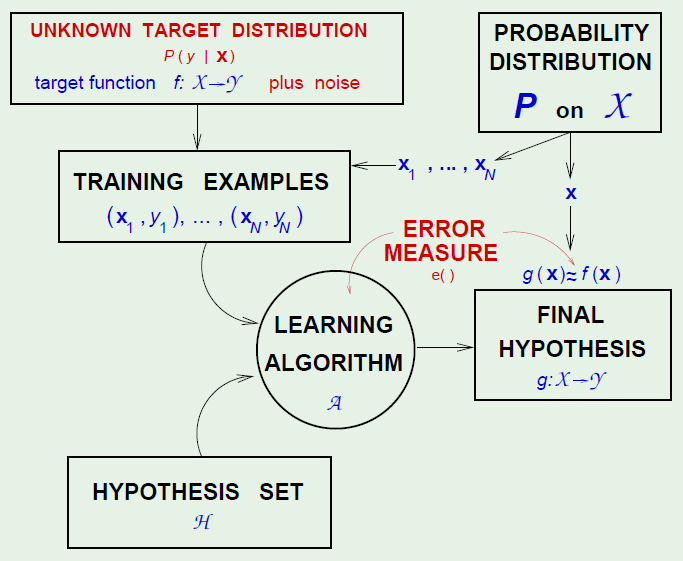
\includegraphics[width=0.6\linewidth]{figure/learning_diagram.png}}
    \caption{The Learning Diagram}\label{fig:learndiag}
\end{figure}

Apparently, the core procedure is learning from sample. We then need to justify that learning from sample is feasible. Hoeffding's inequality provides a theoretical support. It describes the relation between in-sample and out-of-sample error in probabilistic terms. Provided a certain hypothesis $h$,
\begin{equation}\label{eq:hoeffdingtest}
    \mathbb{P}[\vert E_\mathrm{in}(h)-E_\mathrm{out}(h)\vert > \epsilon] \leq 2e^{-2\epsilon^2N}
\end{equation}
where $\epsilon$ is the error term, $N$ is the sample size. One advantage of Hoeffding's inequality is that the bound does not depend on the learning target, which enables it to be applied to all kinds of learning problems.

Note that Inequality \eqref{eq:hoeffdingtest} is an expression of testing, that is, it only works for a given hypothesis. For training we would like to pick the ``best-fitting in-sample" hypothesis in a \textbf{hypothesis set} $\mathcal{H}$. If $\mathcal{H}$ is large enough, it's very likely for us to get a hypothesis with tiny in-sample error. But does it provide a good estimate of out-of-sample error? The answer is most likely NO! We are probably just lucky enough to find one fitting the sample itself very well. Think of $p$-value (the probability of obtaining the observed sample results when the null hypothesis is actually true) as an analogy. If you do an experiment as many times as possible, you will eventually get it right!

Intuitively, we shall involve the size of $\mathcal{H}$ (or equivalently model complexity) in the inequality as a factor of cost. Given a hypothesis set $\mathcal{H}$, in the most conservative case, the experiment for each hypothesis in the set is independent. Hence, we can do a simple summation to obtain the inequality of the hypothesis set (\textit{i.e.} the expression of training),
\begin{equation}\label{eq:hoeffdingtrain}
    \mathbb{P}[\vert E_\mathrm{in}(g)-E_\mathrm{out}(g)\vert > \epsilon] \leq 2\textcolor{red}{M}e^{-2\epsilon^2N}
\end{equation}
where $g$ is a hypothesis picked from $\mathcal{H}$. We will establish later on that relaxing the independence assumption will make learning feasible.

The intuition behind Inequality \eqref{eq:hoeffdingtrain} is that the more hypotheses you try the higher the probability of getting one with very small in-sample error is. $M$ is the price of going through all those hypotheses, and thus, complexity of the hypothesis set $\mathcal{H}$ means a larger $M$. If we have a more complex model, we will fit better in-sample but need more examples (a bigger $N$) to negate the large $M$ in order to satisfy the inequality. The inequality as it is does not offer too much hope since $M$ is often infinity in practice! In the next section, we will introduce a more accurate measure of model complexity to replace $M$ so that the inequality becomes a sound basis for learning feasibility.


\section{Measure of Model Complexity}

From discussion in the previous section, we figured that Inequality \eqref{eq:hoeffdingtrain} is not good enough because $M$ is not a proper measure of model complexity. In order to establish an appropriate measure of model complexity, first we need to introduce the concept of dichotomy. Dichotomy is a partition of a whole (or a set) into two parts (subsets) that are:
\begin{itemize}
    \item jointly exhaustive: everything must belong to one part or the other, and
    \item mutually exclusive: nothing can belong simultaneously to both parts.
\end{itemize}
Such a partition is also frequently called a bipartition.

To better illustrate this concept, let's look at the example of 2-D perceptron. With $N$ points in a two-dimensional space, how many dichotomies can we have at most? The answer is $2^N$, easy enough. However, if we want to do the partition with a straight line, we won't be able to get all $2^N$ dichotomies. And the reason is obvious, that is, our model, straight line, is too simple to capture all possible dichotomies. Hence, although the $M$ is infinite in this case, it doesn't necessarily mean our model is extremely complex. And the uncomplexity is reflected by the limited number of dichotomies the model can achieve. Good news! So we can establish a measure of model complexity based on how many dichotomies the model can get most.

Let's define a measure called Growth Function,
\begin{equation}
    m_\mathcal{H}(N) = \max_{x_1, \dots, x_N \in \mathcal{X}} \vert \mathcal{H}(x_1, \dots, x_N)\vert
\end{equation}
which counts the most dichotomies on any $N$ points for a given model or hypothesis set $\mathcal{H}$. And we can argue that the complexity of a model or hypothesis set can be measured by the growth function.

Note that the growth function must satisfy $m_\mathcal{H}(N) \leq 2^N$ since $2^N$ is the maximum number of dichotomies a data set of size $N$ can possibly have. A fair question is: when does the equality hold? Back to the perceptron example, we can easily show that $m_\mathcal{H}(N) = 2^N$ for $N \leq 3$. If a model (hypothesis set $\mathcal{H}$) can capture all possible dichotomies of a data set, we say that the model or $\mathcal{H}$ can ``shatter" the data set. Thus, a 2-D perceptron can shatter a data set with 3 points at most. Intuitively, a more complex model should be able to ``shatter" data set with more points.

Now we are ready to introduce the key notion of this section -- break point. The \textbf{break point} of a model or hypothesis set $\mathcal{H}$ is the \textcolor{red}{smallest} $k$ where no data set of size $k$ can be shattered by $\mathcal{H}$.

Regarding this very important notion, we need to clarify some potential confusions. First, it's obvious but not trivial to conclude that if $\mathcal{H}$ can shatter no data set of size $k$, it won't be able to shatter any data set of size larger than $k$. Hence, the break point is a critical threshold. Second, an $\mathcal{H}$ with break point $k$ may not be able to shatter all data sets of size smaller than $k$. As we know that the break point for the 2-D perceptron is 4. However, given 3 points on a straight line, the perceptron cannot capture the dichotomy with two points on the sides as one group and the one in the middle as another. But as long as it manages to get all possible combinations for one data set with 3 points, its break point is larger than 3.\footnote{Possible homework: try figure out the break point for different models.}

Both growth function and break point are extremely important measure of model complexity. They are useful in different ways. Growth function is introduced to replace $M$ in the Hoeffding's inequality for training. It must depend on the data set because it measures the cost of training on the data set given certain model. Break point on the other hand, depends only on the model itself. It's useful when we want to determine what model to use given a data set. We would't like a model with large break point if we have a small data set. Think of an extreme case when a model manages to get all possible dichotomies for a data set. It's almost for sure overfitting. Third, a model with infinite break point have $m_\mathcal{H}(N) = 2^N$ for any $N$. Such model is not suitable for learning as it can always fit the sample set perfectly and cannot be generalized to out-of-sample set.

We've been saying that we want to use growth function $m_\mathcal{H}(N)$ to replace $M$. Question is can we really do that? We also need to figure out the form of $m_\mathcal{H}(N)$. It doesn't have to be an explicit expression as long as we can prove that the exponential $e^{-2\epsilon^2N}$ will eventually manage to bring the RHS of Inequality \eqref{eq:hoeffdingtrain} down given a large $N$, so that learning using the hypothesis set $\mathcal{H}$ becomes feasible given enough number of data points. An educated guess is that $m_\mathcal{H}(N)$ (of course $\mathcal{H}$ must have a finite break point) is polynomial. But is it a valid guess? In the next section, we will answer these two questions.


\section{Theory of Generalization}

To summarize, to be able to generalize and show that learning from data is feasible, we need to have two things in place:
\begin{enumerate}
    \item proof that $m_\mathcal{H}(N)$ is polynomial,
    \item proof that $m_\mathcal{H}(N)$ can replace $M$.
\end{enumerate}
Once you have them, negative exponential in Hoeffding's inequality will eventually triumph.

First, let's prove that $m_\mathcal{H}(N)$ is polynomial. Let $B(N,k)$ be the maximum number of dichotomies on $N$ points, with break point $k$.

Replacing $M$ with $m_h(N)$ results in VC inequality formula below, which is arguably the most important equation in machine learning. The inequality helps us to narrow the union bound into Vapnik-Chervonenkis (VC) inequality:
\begin{equation}\label{eq:vc}
    \mathbb{P}[\vert E_{in}(g)-E_{out}(g)\vert > \epsilon] \leq 2m_\mathcal{H}(2N)e^{-1/8\epsilon^2N}
\end{equation}

If there is a break-point for hypothesis set, we are in business. You can have a $g$ such that $E_{in}$ track $E_{out}$ well given large enough sample size. Note that what we talked about is independent of ``target function". This is important, because we do not know and will not know the ``target function".

In the next section, we will discuss in detail the core notion of the whole article -- VC Dimension! The VC dimension of a model in simple terms corresponds to the number of points it can shatter, hence the complexity of the model.


\section{The VC Dimension}

The VC dimension of a hypothesis set $\mathcal{H}$, denoted by $d_{VC}(\mathcal{H})$, is the largest value of $N$ for which $m_\mathcal{H}(N)=2^N$, \textit{i.e.} ``the most points $\mathcal{H}$ can shatter".
If $d_{VC}$ is finite, $g\in H$ will generalize. Note that this is a probabilistic statement in the form of VC Inequality.

In general, think of $d_{VC}$ as the effective number of parameters that you can dial in to get to all dichotomies. Therefore, the VC dimension is a very criterion of choosing the model with proper complexity.

Transform VC inequality into generalization bound:
\begin{equation}
    \mathbb{P}[\vert E_{out}-E_{in} \vert \leq \Omega(N,\mathcal{H},\delta)]\geq 1-\delta
\end{equation}
where $\Omega$ defines how well the model is generalized, and specifically
\begin{equation}
    \Omega(N,\mathcal{H},\delta)=\sqrt{\frac{8}{N}\ln\frac{4m_\mathcal{H}(2N)}{\delta}}
\end{equation}
where $N$ is the sample size; $\mathcal{H}$ is the hypothesis set with certain complexity; $\delta$ is probability of error in VC bound.

We can conclude the following:
\begin{itemize}
    \item A more complex model is better for $E_{in}$ (this is always true) but bad for $\Omega$ and hence for $E_{out}$.
	\item If you want the probability of error to be lower, you will need a higher $N$.
	\item A larger $N$ narrows the gap between $E_{in}$ and $E_{out}$.
\end{itemize}


\section{Bias-Variance Trade-off}

Bias-Variance is a stand-alone theory, but will help us draw a similar conclusion about learning as above.

A small $E_{out}\Longrightarrow$ A good approximation of $f$ out-of-sample.\\
This is primarily what we are interested in.\\
More complex $\mathcal{H}\Longrightarrow$ better chance of approximating $f$, the target function.\\
Many more hypothesis to choose from that would be closer to the target function. But at the same time we need more examples to generalize better as defined by the VC bound!\\
Less complex $\mathcal{H}\Longrightarrow$ better chance of generalization out of sample.\\
Target function might be in the hypothesis set but it will be more difficult to get to that point.

VC analysis approach in the last section shows the generalization bound:
\begin{equation}
    \mathbb{P}[\vert E_\mathrm{out}-E_\mathrm{in}\vert \leq \Omega(N,\mathcal{H},\delta)]\geq 1-\delta
\end{equation}

On the other hand, bias-variance trade-off decomposes $E_{out}$ into ... well ... bias and variance!

Bias defines how well $\mathcal{H}$ can approximate $f$ in the best case scenario. Variance measures how well we can zoom in on a good $h\in \mathcal{H}$.

Two components can be thought as ``approximation" and ``generalization" components. Let's formally define the decomposition:
\begin{equation}
    \mathbb{E}_\mathcal{D}\left[(g^{(\mathcal{D})}(x)-f(x))^2\right] = \underbrace{\mathbb{E}_\mathcal{D}\left[(g^{(\mathcal{D})}(x)-\bar{g}(x))^2\right]}_{\mathrm{var}(x)} + \underbrace{\Big(\bar{g}(x)-f(x)\Big)^2}_{\mathrm{bias}(x)}
\end{equation}
Therefore,
\begin{equation}
\begin{aligned}
    \mathbb{E}_\mathcal{D}\left[E_{out}(g^{(\mathcal{D})})\right] & = \mathbb{E}_x\left[\mathbb{E}_\mathcal{D}\left[(g^{(\mathcal{D})}(x)-\bar{g}(x))^2\right]\right] \\
    & = \mathbb{E}_x[\mathrm{var}(x)+\mathrm{bias}(x)] \\
    & = \mathrm{bias} + \mathrm{var}
\end{aligned}
\end{equation}

In plain terms, how far the hypothesis you formulated given a particular data set differs from the actual target function is broken into two parts:
\begin{itemize}
    \item Variance: How far does the hypothesis differ from best possible hypothesis you can possibly get. Your algorithm navigates through the data set to come up with the hypothesis h. Another set of data points will result in a different hypothesis $h$.
    \item Bias: How far is the best possible $h$ (denoted as $\bar{g}(x)$) from $f$? This is a conceptual tool and does not need to be in the hypothesis set. Note that the bias component does not depend on the data set.
\end{itemize}

Trade-off looks like this:
%\begin{figure}[ht]
%    \begin{minipage}[b]{.5\textwidth}
%        \center{\includegraphics[width=.7\linewidth]{bias}}
%        \caption{Bias}
%    \end{minipage}
%    \begin{minipage}[b]{.5\textwidth}
%        \center{\includegraphics[width=.9\linewidth]{var}}
%        \caption{Variance}
%    \end{minipage}
%\end{figure}

When you go from a small $\mathcal{H}$ to a large $\mathcal{H}$, the bias always decreases because your candidate hypothesis $h$ becomes more complex and thus has the degrees of freedom to mirror the target function $f$ closer. However, variance starts increasing at some point because the $\mathcal{H}$ becomes so complex, the learning algorithm does not have enough data points to navigate successfully. The learning algorithm ends up with $h$'s that are far off from each other. In other terms, you might run into a issue where:
\begin{equation*}
    \mathcal{H}\ \uparrow\ \Longrightarrow\ \mathrm{bias}\ \textcolor{green}{\downarrow}\ \text{but variance}\ \textcolor{red}{\uparrow}
\end{equation*}
Below graph illustrate the bias-variance tradeoff.
%\begin{figure}
%    \center{\includegraphics[width=0.6\linewidth]{tradeoff}}
%    \caption{The Bias-Variance Trade-Off}\label{fig:tradeoff}
%\end{figure}
The bottom line is that you should match the model complexity to the data resources not to the target complexity. If we had more data, variance of the more complex model would be lower but we can't afford this in this case.

Hence, the game in learning is that we should pick a hypothesis set we can afford to navigate in the training set!

Possible Homework: Demonstrate bias-variance tradeoff with $\sin$ curve.


\section{Learning Curves}

In this section, we will illustrate graphically that both approaches above lead to the same conclusions. Particularly, both approaches talk about approximation and generalization.

\subsection{Simple \textit{v.s.} Complex Model}

\begin{itemize}
    \item You need more examples to learn better -read: lower $E_{out}$-.
    \item The parallel line is the bias. Notice that the bias is lower for the more complex model.
    \item On the flip side, if you have only few examples, you should clearly see that you cannot afford to use a complex algorithm. Your $E_{in}$ will be lower but any hopes of learning from data will get bashed by a large $E_{out}$.
        \begin{itemize}
            \item In VC bound terms, the $\Omega$ is large because of the complexity of the model.
            \item In bias-variance terms, your bias is lower, but your variance is super high because you don't have enough data points.
        \end{itemize}
    \item Also notice that $E_{in}$ can be zero if you have a complex enough model and not a lot of data points. The model in this case will memorize everything. But as seen in the figure, this does not translate well into $E_{out}$.
    \item You need more examples for the more complex model. If you don't, use a simpler model. Remember: the game in learning is that we should pick a hypothesis set we can afford to navigate in the training set!
\end{itemize}

%\begin{figure}[ht]
%    \begin{minipage}[b]{.5\textwidth}
%        \center{\includegraphics[width=.9\linewidth]{SimpleModel}}
%        \caption{Simple Model}
%    \end{minipage}
%    \begin{minipage}[b]{.5\textwidth}
%        \center{\includegraphics[width=.9\linewidth]{ComplexModel}}
%        \caption{Complex Model}
%    \end{minipage}
%\end{figure}

\subsection{VC-Dimension \textit{v.s.} Bias-Variance Approach}

\begin{itemize}
    \item Bias depends on the complexity of the model (not on the data set in hand) and hence constant. It is the best you can do in theory given the hypothesis set.
    \item If you have a more complex model, in the absence of sufficient data points, $\Omega$ will drive the $E_{out}$ to the moon even though $E_{in}$ goes down.
    \item more complex the model $\Longrightarrow\ E_{in}\ \downarrow\ \mathrm{but}\ \Omega\ \uparrow$.
\end{itemize}

%\begin{figure}[ht]
%    \begin{minipage}[b]{.5\textwidth}
%        \center{\includegraphics[width=.9\linewidth]{VCAnalysis}}
%        \caption{VC Analysis}
%    \end{minipage}
%    \begin{minipage}[b]{.5\textwidth}
%        \center{\includegraphics[width=.9\linewidth]{BiasVariance}}
%        \caption{bias-variance}
%    \end{minipage}
%\end{figure}


\section{Overfitting}

Overfitting, in simplest terms, is fitting the data more than warranted. The culprit is fitting the noise.
Think of two logistic regression models; one with 2 variables and the other one with 10 variables.
The latter model will always fit better in-sample. However, if the out-of-sample error of the complex more is higher than the simpler one in a given exercise, we say that the complex model is overfitting. More complex model only loses (and overfits) because number of samples is inadequate. In other terms, overfitting happens when $E_{out}\ \uparrow$ even though $E_{in}\ \downarrow$.

%\begin{figure}
%    \center{\includegraphics[width=0.6\linewidth]{overfitting}}
%    \caption{Overfitting}\label{fig:overfitting}
%\end{figure}

\subsection{Noise}

Noise can be though in two parts: deterministic noise and stochastic noise. So far we have not touched upon the complexity of the target function. Deterministic noise is part of target complexity that our $\mathcal{H}$ cannot capture. We are more susceptible to detect a false pattern given the limitations. As far as we are concerned, this unexplainable part is not any different than the stochastic Gaussian noise.

\subsection{Bias-Variance Framework}

We can also approach the problem from a bias-variance framework. As you recall, bias is a function of your hypothesis set and does not depend on the training data. In that light, deterministic noise is how short your best hypothesis falls of the target. Bias is the direct impact of the noise. Problem of overfitting shows up in the form a high variance. The noise effects the variance by making the model blindly follow the noise unable to distinguish noise from signal. The algorithm will try to fit both types of noise, which is out of reach, which will lead to a high variance.
Going back to our two models:
\begin{enumerate}
    \item Logistic Regression with 2 variables will have a higher bias but lower variance,
    \item Logistic Regression model with 10 variables will have a lower bias but higher variance.
\end{enumerate}

%\begin{figure}[ht]
%    \begin{minipage}[b]{.5\textwidth}
%        \center{\includegraphics[width=.9\linewidth]{overfith2}}
%        \caption{$\mathcal{H}_2$}
%    \end{minipage}
%    \begin{minipage}[b]{.5\textwidth}
%        \center{\includegraphics[width=.9\linewidth]{overfith10}}
%        \caption{$\mathcal{H}_10$}
%    \end{minipage}
%\end{figure}

An analogy might be a person finding herself in an unfamiliar forest with a partial map. Every time she starts her expedition to find her way out, she will end up at a different place (high variance), because she does not have the toolkit to deal with the complexity of the forest. Solution can be (1) studying forestry to understand the ecosystem etc better, or (2) acquiring a more complete map. In our example, the first solution is analogous to a more complex hypothesis set, whereas second solution can be thought as working with more data points.

In short, the interaction of $\mathcal{H}$ with $N$ determines the variance, hence the overfitting problem. This is another way of stating that we should pick a hypothesis set we can afford to navigate in the training set!

Summarizing the somehow wordy explanation:
\begin{itemize}
    \item $N\ \uparrow\ \Longrightarrow\ \mathrm{Overfitting}\ \downarrow$
    \item Deterministic Noise $\uparrow\ \Longrightarrow\ \mathrm{Overfitting}\ \uparrow$
    \item Stochastic Noise $\uparrow\ \Longrightarrow\ \mathrm{Overfitting}\ \uparrow$
\end{itemize}

How do we deal with overfitting is explained in the next section.


\section{Regularization and Cross Validation}

\subsection{Regularization}

Putting in a regularizer is inevitable in almost in all machine learning situations. Regularization reduces variance at the expense of bias and introduces a simpler hypothesis by limiting the weights of the parameters. As a practical rule, the noise is higher-frequency than the signal. Constraining learning towards smaller hypothesis punishes noise more than signal. Smaller weights often correspond to smaller functions.

The graph below illustrates the impact of introduction of regularization. In the absence of regularization, the $w_{lin}$ minimizes the in-sample error. Introduction of the regularization constraint (red circle) prohibits us going all the way to $w_{lin}$.
%\begin{figure}
%    \center{\includegraphics[width=0.4\linewidth]{regularize}}
%    \caption{Impact of Regularization}\label{fig:regularize}
%\end{figure}

Formally, $\lambda$ is the ``hyper-parameter" of the model. A more restricted model or a smaller $C$ (radius of the circle) corresponds to a larger $\lambda$.

Minimize
\begin{equation*}
    E_\mathrm{in}(w)+\frac{\lambda}{N}w^Tw
\end{equation*}
\[
\boxed{C\ \uparrow\ \ \lambda\ \downarrow}
\]
The new error term is called ``augmented error" and is better than $E_\mathrm{in}$ as a proxy of $E_\mathrm{out}$. Introduction of the hyper-parameter takes us one step closer to the holy grail of machine learning, finding an in-sample estimate of the out-of-sample error.

The $E_\mathrm{aug}$ error term is analogous to generalization bound we derived from VC inequality. Both equations explicitly penalize for model complexity through overfit penalty.

Calling the regularizer $\Omega=\Omega(h)$, we minimize
\[
    \textcolor{purple}{E_\mathrm{aug}}(h) = \textcolor{blue}{E_\mathrm{in}}(h) + \frac{\lambda}{N}\Omega(h)
\]
Rings a bell?
\[
    \downarrow\ \ \downarrow
\]
\[
    \textcolor{red}{E_\mathrm{out}}(h) \leq \textcolor{blue}{E_\mathrm{in}}(h) + \Omega(\mathcal{H})
\]

Choosing the term $\Omega$ is a heuristic choice guided by theory and certain goals. Two very common regularization techniques are L1 and L2 norms:

L1 regularization: $\min(\Vert y-x\beta\Vert^2 + \lambda\Vert x\Vert)$

L2 regularization: $\min(\Vert y-x\beta\Vert^2 + \lambda\Vert x\Vert^2)$

On the other hand, validation helps us to determine the right dosage of hyper-parameter in our model.

\subsection{Validation}

While regularization is mainly about estimating the overfit penalty, validation looks at the bottom line by estimating $E_\mathrm{out}$. It is called 'validation' because we use it to make choices.

\[
    E_\mathrm{out}(h) = E_\mathrm{in}(h) + \mathrm{overfit\ penalty}
\]

Regularization:
\[
    E_\mathrm{out}(h) = E_\mathrm{in}(h) + \underbrace{\mathrm{overfit\ penalty}}_{\textcolor{red}{\mathrm{estimated\ by\ regularization}}}
\]
Validation:
\[
    \underbrace{E_\mathrm{out}(h)}_{\textcolor{red}{\mathrm{estimated\ by\ validation0}}} = E_\mathrm{in}(h) + \mathrm{overfit\ penalty}
\]

Let's call the data set $\mathcal{D}=\{(x_1,y_1),\dots,(x_N,y_N)\}$, and the number of data points in the validation set $K$. The number of data points in the training set is therefore $N-K$.

We can show that $E_\mathrm{val}$ is an unbiased estimator of $E_\mathrm{out}$ because we have not seen the data points in the validation set while training our model. You can see that the variance of the estimate depends on $K$. The larger the $K$, the smaller the variance of the estimate will be. Ideally, we want a small variance, hence a large $K$.

\[
    \mathbb{E}\left[E_\mathrm{val}(h)\right] = \frac{1}{K} \displaystyle\sum_{k=1}^K\mathbb{E}\left[ e(h(x_k),y_k) \right] = E_\mathrm{out}(h)
\]
\[
    \mathrm{var}\left[E_\mathrm{val}(h)\right] = \frac{1}{K^2} \displaystyle\sum_{k=1}^K\mathrm{var}\left[ e(h(x_k),y_k) \right] = \frac{\sigma^2}{K}
\]

However, $K$ is not free. You borrow $K$ points away from the training set. Why does this matter? To answer the question, let's go back to learning curves. While a large $K$ all but ensures that we have a reliable estimate but at the expense of model performance. In other words, I am getting a reliable estimate of a worse quantity as $K$ get larger.

%\begin{figure}
%    \center{\includegraphics[width=0.5\linewidth]{validation}}
%    \caption{Number of data points for validation}\label{fig:validation}
%\end{figure}

\subsection{Model Selection Using Validation}

Choosing a parameter with validation introduces bias because you pick the model with lower $E_\mathrm{val}$. It is the minimum error on one set of realization of data points. We should concede that bias is not going to hurt us much. But we need to be careful with keeping the validation set fairly clean or not very contaminated.
In formal terms, the generalization bound applies to this particular problem. $M$ below denotes number of parameters to choose in the validation exercise.
\begin{equation}
    E_\mathrm{out}(\bar{g_{m^*}}) \leq E_\mathrm{val}(\bar{g_{m^*}}) + O\large(\sqrt{\frac{\ln\textcolor{red}{M}}{K}}\large)
\end{equation}

\subsection{Cross-Validation}

Now that we have taken care of the reliability of the validation set, let's go back to the selection of $K$. We have the following dilemma with the selection of $K$. We want a large $K$ to have a reliable out-of-sample estimate, in the meantime we want a small $K$ to have a robust model.

Can $K$ be equal to both small and large?
\begin{gather*}
    E_\mathrm{out}(g) \approx E_\mathrm{out}(g\bar{\ }) \approx E_\mathrm{val}(g\bar{\ }) \\
    \textcolor{red}{(\text{small}\ K)\ \ \ (\text{large}\ K)}
\end{gather*}

Leave-one-out validation helps us to get there.
$N-1$ training set and 1 point for validation. The common point between all the little guys is that they are out of sample with respect to the hypothesis they try evaluate, unbiased, and trying to estimate the same thing. Repeat the process $N$ times.

The common thread among all the hypothesis is that they are obtained by training on $N-1$ data points. Because of the learning curve, we know there is a tendency.The fact that they all come from $N-1$ data points tells me that they are realizations of something that is the expected value of all them. The little guys are trying to estimate the same thing as a result.

You will notice that, all of a sudden, the validation set looks quite respectable with N examples. This comes on top of the fact that I was able to use $N-1$ to train. The catch is $e$'s are not independent. Surprisingly, the method is remarkably efficient in getting there.

$N-1$ points for training, and \textcolor{red}{1 point} for validation!
\[
    \mathcal{D}_n = (\mathbf{x}_1,y_1), \dots, (\mathbf{x}_{n-1},y_{n-1}), \textcolor{red}{\cancel{(\mathbf{x}_n,y_n)}}, (\mathbf{x}_{n-1},y_{n-1}), \dots, (\mathbf{x}_N,y_N)
\]
Final hypothesis learned from $\mathcal{D}_n$ is $\bar{g_n}$
\[
    e_n = E_\mathrm{val}(\bar{g_n}) = e(\bar{g_n}(\mathbf{x}_n,y_n))
\]
Cross-validation error:
\[
    E_\mathrm{CV} = \frac{1}{N}\sum_{n=1}^Ne_n
\]


\end{document}
